\documentclass[12pt,a4paper]{article}

\usepackage[utf8]{inputenc}
\usepackage[T1]{fontenc}
\usepackage[english]{babel}
\usepackage{lmodern}
\usepackage[margin=2.6cm]{geometry}
\usepackage{amsmath,amssymb}
\usepackage{booktabs}
\usepackage{graphicx}
\usepackage{float}
\usepackage{listings}
\usepackage{xcolor}
\usepackage[hidelinks]{hyperref}

\graphicspath{{../figures/}}

\lstset{basicstyle=\ttfamily\small, frame=single, breaklines=true,
        columns=fullflexible, backgroundcolor=\color{gray!8}}

\setlength{\emergencystretch}{3em}

\newcommand{\act}[1]{\texttt{#1}}

\title{Process Mining and Formal Verification of the\\
       Volvo IT Incident Management Process\\
       \large BPI Challenge 2013}
\author{Francesco Sgaramella}
\date{\today}

\begin{document}
\maketitle

\begin{abstract}
This report analyses the BPI Challenge 2013 event logs from Volvo IT Belgium's
VINST incident and problem management system. Three discovery algorithms are
compared, model quality is assessed on four conformance dimensions, and eight
temporal properties are verified against every case using finite-trace linear
temporal logic. Three findings emerge. Rework dominates the process: fewer than
half of all recorded events are the first occurrence of their activity within a
case. The documented procedure of queueing an incident before working it is
violated in the large majority of cases, a deviation established by formal
verification rather than by inspection. And the Alpha miner fails on this log, defeated by the loop behaviour of the
process.
\end{abstract}

\section{Introduction}

\subsection{Context}

This report applies process discovery, conformance checking and formal
verification to the BPI Challenge 2013 dataset: the incident and problem
management logs of Volvo IT Belgium, recorded by the VINST service management
system.
\subsection{Objectives}

\begin{enumerate}
  \item Derive process models from the logs using three discovery
        algorithms and compare them using metrics.
  \item Specify properties of the incident process in temporal logic and verify
        them against every recorded case.
  \item Quantify where time is spent and identify the structural sources of
        delay.
  \item Determine whether the process as executed matches the process as
        documented.
\end{enumerate}

\section{Theoretical foundations}\label{sec:foundations}

\subsection{Event logs}

An event log is a multiset of traces. A trace is a finite sequence of events
belonging to one case, ordered by timestamp; each event carries at minimum a
case identifier, an activity name and a timestamp. Writing $\Sigma$ for the set
of activities, a trace is an element of $\Sigma^*$ and a log is a multiset over
$\Sigma^*$. Two traces with the same activity sequence belong to the same
variant, so few variants means a standardised process.

\subsection{Petri nets}

A Petri net models the control flow of a log. Different discovery techniques
extract that flow from the recorded events.

\subsection{Conformance dimensions}

Four dimensions are used to compare the discovered Petri nets.

\begin{description}
  \item[Fitness] The extent to which the model can replay the traces in the log.
        A fitness of $1$ means every observed case is replayable.
  \item[Precision] The extent to which the model forbids behaviour
        that never occurred. Low precision indicates an over-permissive model.
  \item[Generalisation] The extent to which the model is expected to accommodate
        future behaviour rather than being overfitted to the observed traces.
  \item[Simplicity] A structural measure penalising the complexity of the net.
\end{description}

\subsection{Linear temporal logic over finite traces}\label{sec:ltlf}

Properties of traces are expressed in linear temporal logic. Because a case is a
finite sequence of events, the semantics used here are those of linear temporal
logic interpreted over finite traces.

\section{The dataset}\label{sec:dataset}

\subsection{Origin and scale}

The BPI Challenge 2013 data comprises three logs recorded by Volvo IT Belgium's
VINST system: one of incidents, and two of problems, divided into those open and
those closed at the time of extraction.

\begin{table}[H]
\centering
\begin{tabular}{lrrrll}
\toprule
Log & Cases & Events & Activities & From & To \\
\midrule
closed\_problems & 1,487 & 6,660 & 7 & 2006-01-11 & 2012-05-31 \\
incidents & 7,554 & 65,533 & 13 & 2010-03-31 & 2012-05-22 \\
open\_problems & 819 & 2,351 & 5 & 2006-11-07 & 2012-06-15 \\
\bottomrule
\end{tabular}

\caption{The three Volvo IT Belgium's VINST system logs comparison}
\label{tab:dataset}
\end{table}

The incident log is the principal object of study; the problem logs are used for
comparison in Section~\ref{sec:health}. They are not variants of one process.

\subsection{The activity label is a modelling decision}\label{sec:mode}

Each event records a \act{Status} and a
\act{Sub Status}. The two can be treated as one composite label or as independent
dimensions; the composite choice increases the complexity of the resulting Petri
net.

\begin{figure}[H]
\centering
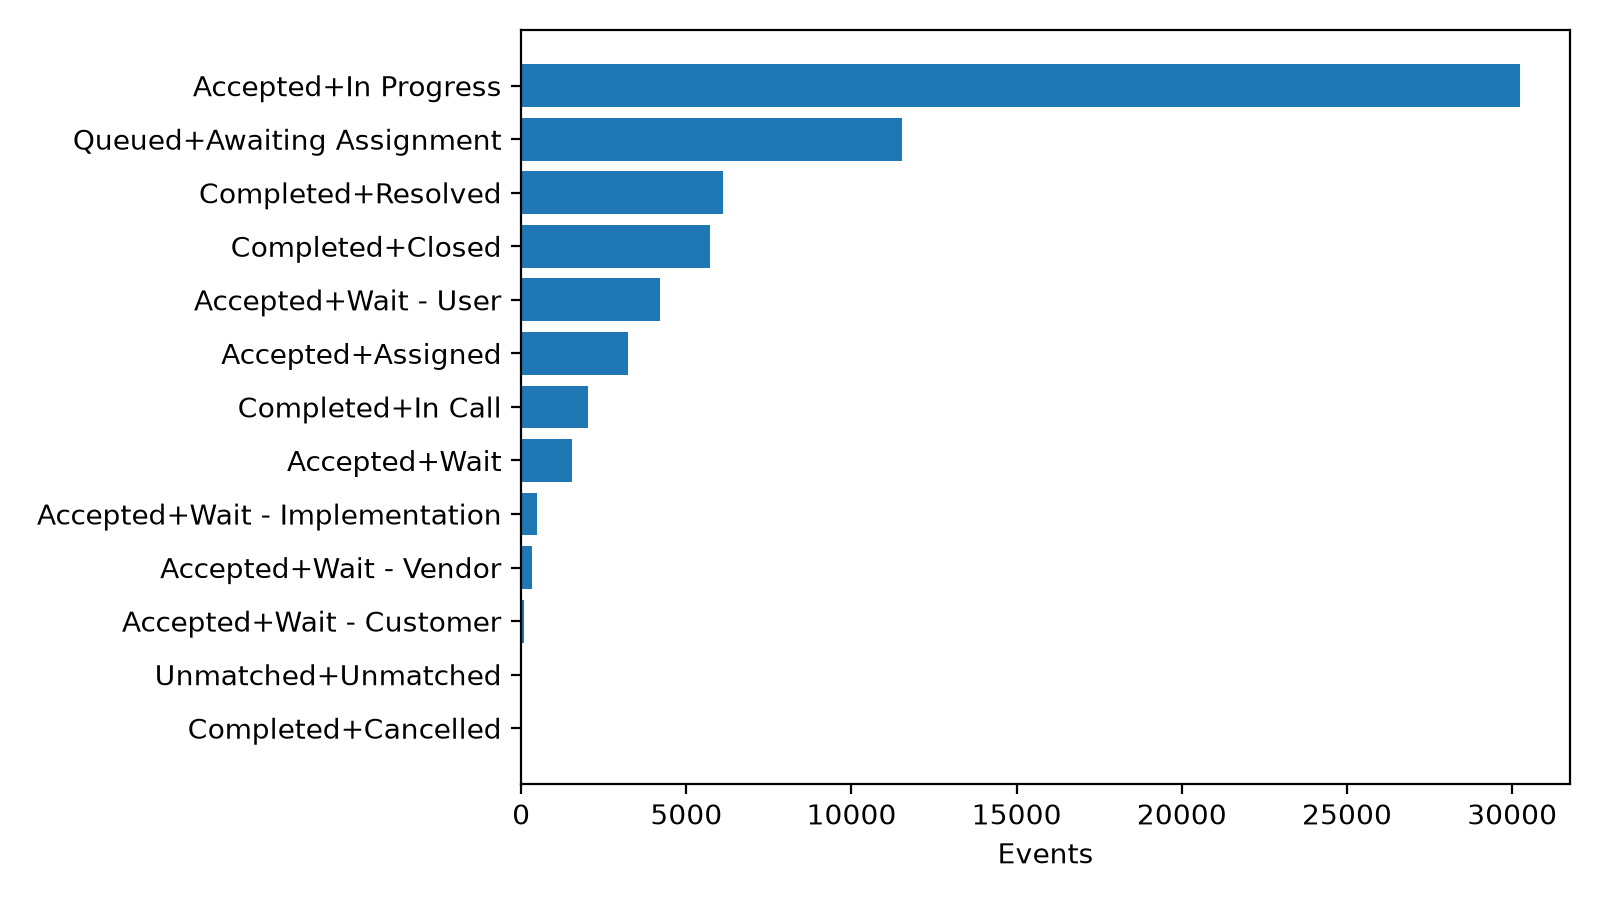
\includegraphics[width=0.68\textwidth]{activity_frequency.png}
\caption{Event counts per activity in the incident log under the composite
labelling. \act{Accepted+In Progress} accounts for the plurality of all events.}
\label{fig:activity-frequency}
\end{figure}

\section{Process discovery}\label{sec:discovery}

\subsection{Algorithms}

Three algorithms are compared.

\begin{description}
  \item[Alpha miner] Infers ordering relations from consecutive states and
        constructs a net from them. It does not handle noise and loops.
  \item[Heuristics miner] Uses consecutive states frequency and
        applies a dependency threshold, so infrequent behaviour is filtered out.
  \item[Inductive miner] Uses trees that are converted into graphs to model the net. Guarantees soundness and, at a noise threshold of zero, perfect fitness.
\end{description}

\subsection{Results}

\begin{table}[H]
\centering
\small
\begin{tabular}{llrrrrrr}
\toprule
Mode & Algorithm & Fitness & Precision & Gen. & Simpl. & Places & Trans. \\
\midrule
status & alpha & 0.119 & 0.400 & 0.734 & 1.000 & 2 & 4 \\
status & heuristics & 0.994 & 0.678 & 0.767 & 0.622 & 8 & 15 \\
status & inductive & 1.000 & 0.440 & 0.748 & 0.667 & 17 & 23 \\
status+substatus & alpha & 0.127 & 0.176 & 0.770 & 0.789 & 2 & 13 \\
status+substatus & heuristics & 0.948 & 0.387 & 0.634 & 0.471 & 27 & 69 \\
status+substatus & inductive & 1.000 & 0.234 & 0.783 & 0.634 & 57 & 78 \\
\bottomrule
\end{tabular}

\caption{Discovery on the full incident log; conformance computed on a sample of
cases. Both activity labellings are shown.}
\label{tab:discovery}
\end{table}

Three observations follow.

\paragraph{The fitness and precision trade off.} The Inductive miner
attains perfect fitness but loses precision: it buys replayability by being
permissive, and it produces by far the largest net. The Heuristics miner sacrifices a little
fitness for substantially better precision in a net a fraction of the size.

\paragraph{The Alpha miner fails.}
Its fitness falls below $0.15$ in both labellings and the net degenerates to two
places. Loops are the cause: ninety percent of cases in this log contain at
least one length-one loop, which the Alpha miner provably cannot represent.

\paragraph{Finer labels cost precision.} Moving from four activities to thirteen
lowers precision for every algorithm and roughly triples model size, for the
reason given in Section~\ref{sec:mode}.

\begin{figure}[H]
\centering
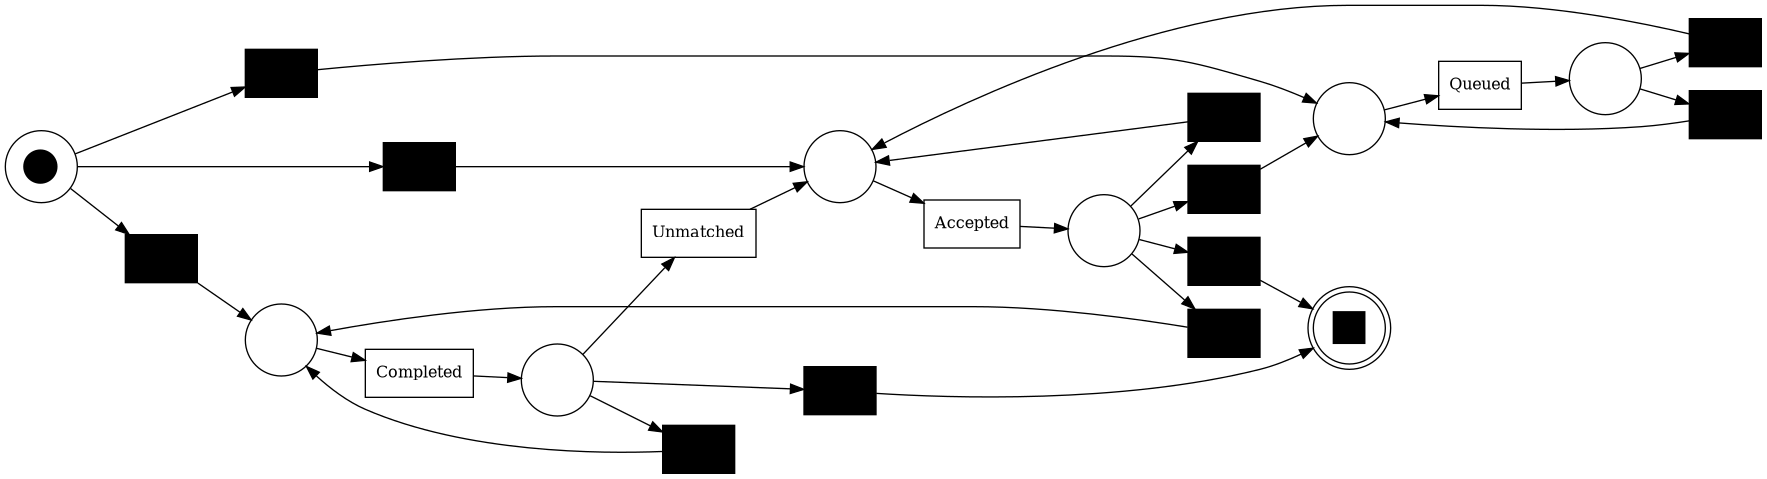
\includegraphics[width=0.62\textwidth]{petri_heuristics_status.png}
\caption{Heuristics miner, \act{Status} labelling. The best-balanced model of
those compared.}
\label{fig:petri-heuristics}
\end{figure}

\begin{figure}[H]
\centering
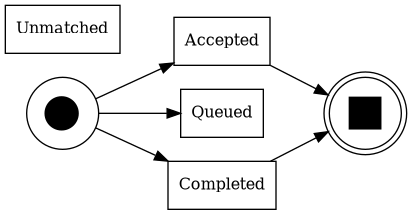
\includegraphics[width=0.45\textwidth]{petri_alpha_status.png}
\caption{Alpha miner, \act{Status} labelling. The degenerate structure is the
consequence of length-one loops, not of noise in the data.}
\label{fig:petri-alpha}
\end{figure}

\section{Performance analysis}\label{sec:performance}

\subsection{Method}

Waiting time is measured as the interval between an event and the next event of
the same case. The last event of a case has no successor and is therefore
excluded.

\begin{table}[H]
\centering
\small
\begin{tabular}{lrrrr}
\toprule
Activity & n & Mean (h) & Median (h) & Max (h) \\
\midrule
Completed+Closed & 143 & 143.31 & 95.28 & 736.50 \\
Accepted+Wait - Vendor & 313 & 131.63 & 28.15 & 1633.67 \\
Accepted+Wait - Implementation & 491 & 130.22 & 26.00 & 3500.55 \\
Accepted+Wait - Customer & 101 & 115.45 & 54.39 & 1488.93 \\
Completed+Resolved & 6,025 & 114.15 & 176.25 & 192.10 \\
Accepted+Wait - User & 4,214 & 109.97 & 26.36 & 5059.88 \\
Accepted+Wait & 1,533 & 97.99 & 3.45 & 4992.31 \\
Completed+In Call & 153 & 70.88 & 1.56 & 677.31 \\
Accepted+Assigned & 3,220 & 36.31 & 1.36 & 17334.07 \\
Queued+Awaiting Assignment & 11,544 & 26.16 & 0.59 & 6838.52 \\
Accepted+In Progress & 30,237 & 10.63 & 0.03 & 7896.28 \\
Unmatched+Unmatched & 5 & 0.19 & 0.07 & 0.61 \\
\bottomrule
\end{tabular}

\caption{Waiting time after each activity in the incident log. Both mean and
median are reported; see below for why either alone misleads.}
\label{tab:waiting}
\end{table}

\subsection{Mean and median diverge}

For \act{Accepted+In Progress} the median waiting time is on the order of
minutes while the mean is on the order of hours. The work is normally picked up immediately and occasionally stalls for
a very long time. Both are reported to show the phenomenon.

\begin{figure}[H]
\centering
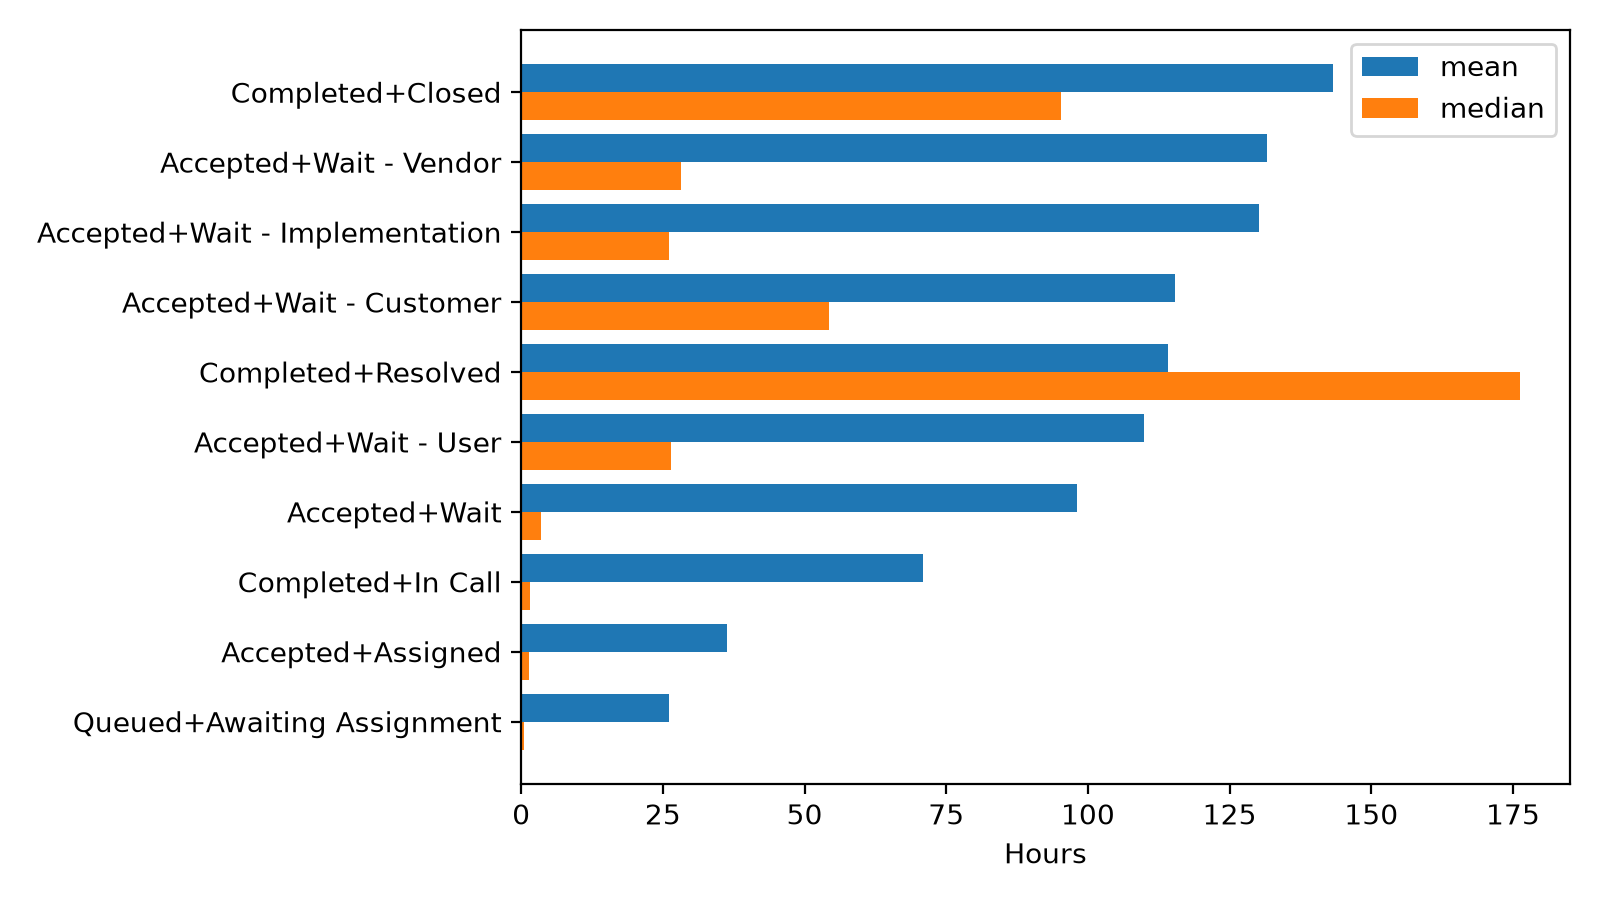
\includegraphics[width=0.68\textwidth]{waiting_times.png}
\caption{Mean against median waiting time for the slowest activities. Where the
bars diverge sharply, the activity is usually fast and occasionally pathological.}
\label{fig:waiting}
\end{figure}

\subsection{Where the time goes}

The \act{Wait} states dominate mean waiting time characteristic for a support process whose delays are
external rather than internal, and it locates the improvement opportunity
outside the service desk itself.

That \act{Completed+Closed} appears in Table~\ref{tab:waiting} at all means a
substantial number of closure events were \emph{not} the last event of their
case: work continued after the incident was formally closed.
Section~\ref{sec:verification} reaches the same conclusion by another route.

\subsection{Duration and variability}

\begin{figure}[H]
\centering
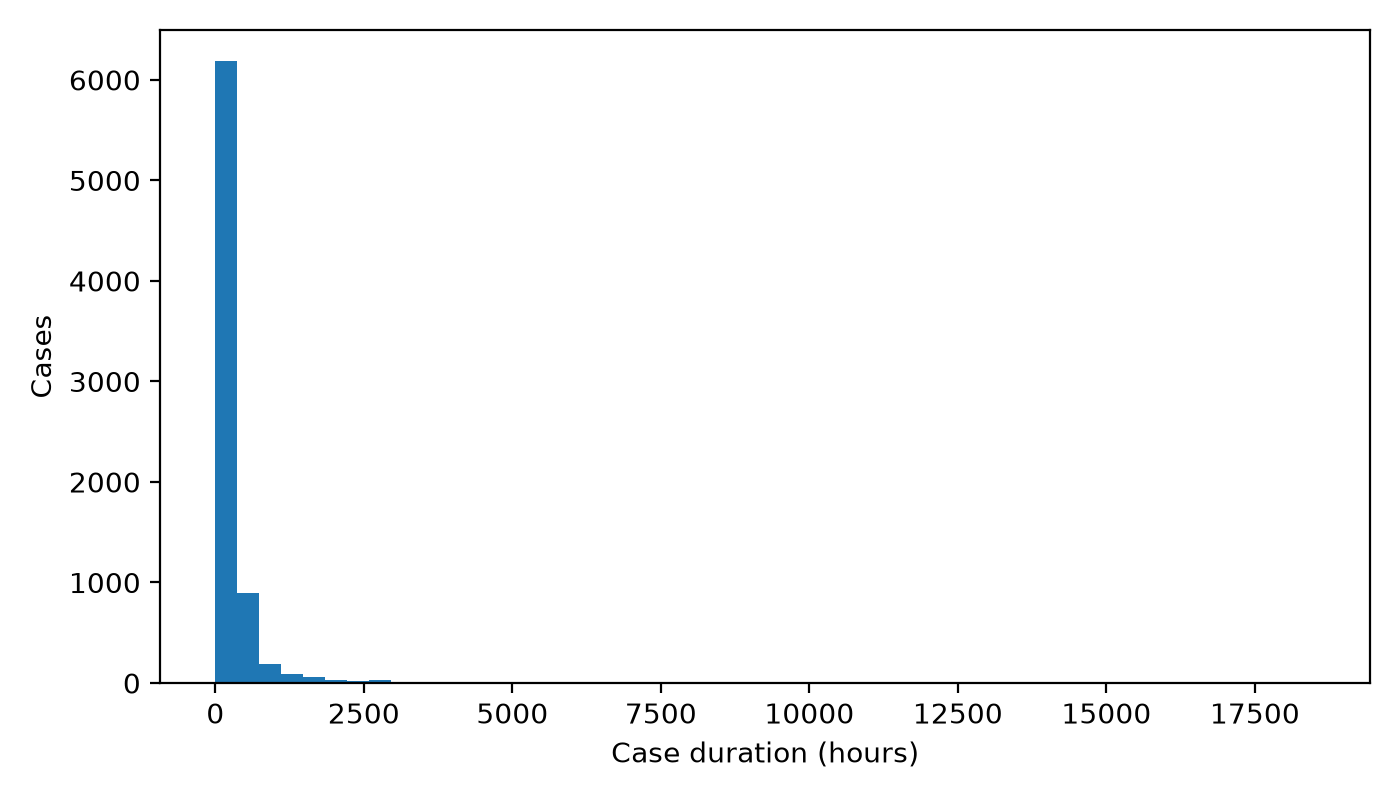
\includegraphics[width=0.52\textwidth]{duration_hist.png}
\caption{Distribution of case durations in the incident log.}
\label{fig:duration}
\end{figure}

\begin{figure}[H]
\centering
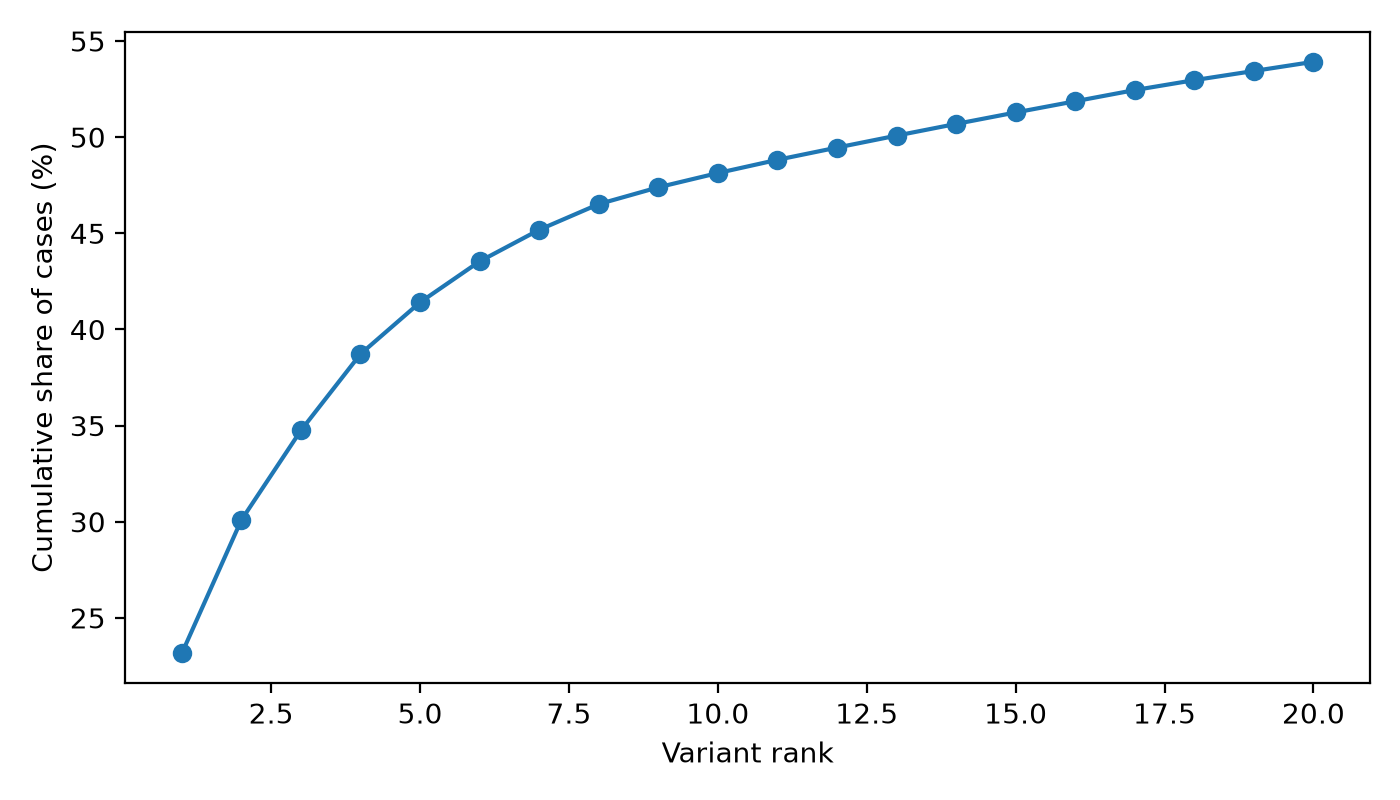
\includegraphics[width=0.52\textwidth]{variant_pareto.png}
\caption{Cumulative share of cases covered by the most frequent variants. The
curve flattens early: a large minority of cases follow paths that occur once.}
\label{fig:pareto}
\end{figure}

The process is only weakly standardised. Distinct variants number in the
thousands against seven and a half thousand cases, and the majority of variants
occur exactly once. Any model of this log with high precision would be
overfitted, which is the proper interpretation of the precision figures in
Table~\ref{tab:discovery}.

\section{Formal verification}\label{sec:verification}

\subsection{Specification}

Eight properties were specified in temporal logic over the composite activity
alphabet, with activity labels mapped to proposition symbols
(\act{Accepted+In Progress} becomes \texttt{accepted\_in\_progress}). Each is
evaluated independently against every case; the satisfaction ratio is the share
of cases satisfying it, and violating cases are retained as counterexamples. Six
properties express expectations that ought to hold; two express the documented
procedure and are included because they are expected to fail, the size of the
gap being the result.

\begin{table}[H]
\centering
\small
\begin{tabular}{lrrr}
\toprule
Property & Satisfied & Violated & Ratio \\
\midrule
Termination & 7,546 & 8 & 0.999 \\
Resolution & 7,545 & 9 & 0.999 \\
No work after closure & 7,435 & 119 & 0.984 \\
Queued work is picked up & 7,494 & 60 & 0.992 \\
Waiting on the user resumes & 7,550 & 4 & 0.999 \\
No unmatched events & 7,549 & 5 & 0.999 \\
Formal closure & 5,591 & 1,963 & 0.740 \\
Queueing precedes work & 1,168 & 6,386 & 0.155 \\
\bottomrule
\end{tabular}

\caption{Verification against all cases of the incident log.}
\label{tab:ltl}
\end{table}

\subsection{Interpretation}

\paragraph{The process terminates and resolves.} Termination, resolution, and
recovery from waiting on the user each hold for essentially every case. Whatever
else is wrong with this process, cases do not disappear into it.

\paragraph{Work continues after closure.} The property
\[
  \mathbf{G}\,(\texttt{completed\_closed} \rightarrow
  \neg\mathbf{F}\,\texttt{accepted\_in\_progress})
\]
fails for a small but non-trivial number of cases: an incident is formally
closed and then worked again, corroborating the appearance of
\act{Completed+Closed} in the waiting-time table of
Section~\ref{sec:performance}.

\paragraph{Formal closure is not universal.} A quarter of incidents that are
worked never reach \act{Completed+Closed}; they are settled as
\act{Completed+In Call} instead.

\paragraph{Queueing does not precede work.} The documented procedure is that an
incident is queued for assignment and then taken up. Formally,
\[
  (\neg\,\texttt{accepted\_in\_progress}) \;\mathbf{U}\;
  \texttt{queued\_awaiting\_assignment}.
\]
This holds for a small minority of cases. In the large majority, work begins
without the incident ever having been queued.

\subsection{A methodological result: strong next}\label{sec:strongx}

The no-work-after-closure property was first written in the form
\[
  \mathbf{G}\,(\texttt{completed\_closed} \rightarrow
  \mathbf{X}\,\mathbf{G}\,\neg\,\texttt{accepted\_in\_progress}),
\]
the natural infinite-trace formulation, which reports a satisfaction ratio of
roughly one quarter, an apparently severe process failure. The figure is an
artefact: $\mathbf{X}$ is false at the final position of a finite trace
(Section~\ref{sec:ltlf}) and most cases here \emph{end} with
\act{Completed+Closed}, falsifying the implication for reasons unrelated to the
process. The $\mathbf{F}$-based formulation above avoids $\mathbf{X}$ and
reports the true figure of roughly $98\%$.

\section{Aggregate assessment}\label{sec:health}

To compare the three logs on one scale, a composite score aggregates four
normalised components: the share of cases reaching a completed state; the share
of events that are the first occurrence of their activity within their case;
one minus the variant ratio; and a throughput term derived from median case
duration against a fixed horizon.

\begin{table}[H]
\centering
\small
\begin{tabular}{lrlrrrr}
\toprule
Log & Score & Grade & Completion & Rework & Standardisation & Throughput \\
\midrule
closed\_problems & 65.9 & D & 1.000 & 0.655 & 0.780 & 0.000 \\
incidents & 74.4 & C & 0.999 & 0.481 & 0.698 & 0.748 \\
open\_problems & 70.0 & D & 0.435 & 0.746 & 0.778 & 0.942 \\
\bottomrule
\end{tabular}

\caption{Composite score and its components across the three logs. Higher is
better on every component.}
\label{tab:health}
\end{table}

The weighting and the throughput horizon are stipulated, so the score compares
logs and labellings but carries no absolute meaning. Completion is near perfect
and variability moderate, but fewer than half of all events are first
occurrences of their activity: over half of the recorded work in the incident
process is repetition.

\section{Implementation}\label{sec:architecture}

The analysis is a single self-contained Python package; dependencies are
declared in \texttt{pyproject.toml} and resolved with \texttt{uv}. The results
reported here were produced with Python 3.12, pm4py 2.7.23, flloat 0.3.0,
pandas 3.0 and Graphviz 2.43, with Gradio 6.26 for the dashboard and Matplotlib
3.11 for the figures. The language model clients are an optional extra.

\texttt{logs.loader.load} detects the schema, derives the activity label and
returns an \texttt{EventLogBundle} carrying the pm4py log, the full source
frame, the schema and the labelling mode. Normalisation \emph{adds} the
XES-standard columns rather than reducing each event to them, preserving the
support-line, ownership and country attributes that Section~\ref{sec:threats}
identifies as the basis of any continuation of this work. The label is computed
here from the \act{Status} and \act{Sub Status} pair, under a mode that is a
parameter of \texttt{load} and is then frozen into the bundle: the single point
at which the modelling decision of Section~\ref{sec:mode} enters the system, and
what allows the same log to be loaded twice under different labellings and the
two models compared.

Verification encodes each case as one finite word. Since activity labels are not
valid proposition symbols, \texttt{verification.ltl.Alphabet} maps them to
identifiers (\act{Accepted+In Progress} becomes
\texttt{accepted\_in\_progress}) and gives each position a total truth
assignment, as flloat requires. A symbol absent from the log is padded to false
throughout; strict parsing rejects a symbol that names no activity anywhere in
the dataset, separating a genuinely absent activity from a mistyped one. The
eight named properties are declared as data and evaluated by the same function
that evaluates a formula typed into the dashboard.

The dashboard exposes the same analyses interactively across ten panels. Beyond
the discovery, conformance, verification and performance results reported above,
three of them are exploratory rather than confirmatory. Preprocessing composes
the filters of \texttt{logs.preprocessing} in a fixed order --- activities, time
range, case length, duplicates, relabelling --- so that a result does not depend
on the order in which the controls were operated; each application replaces the
session log, and reloading restores it. The anomaly panel reports the four
statistical outlier families of \texttt{analysis.anomalies} --- case lengths
beyond a chosen number of standard deviations, activities below a share of all
events, waits beyond a duration, and transitions below a support --- with every
threshold exposed as a control, since each is a modelling choice rather than a
property of the log. The prediction panel fits the first-order Markov model of
\texttt{analysis.predictor} that also produces the transition heatmap of
Section~\ref{sec:performance}, and reports successor probabilities and the
greedy most-likely continuation from a chosen activity; the Markov assumption
makes a long walk indicative rather than a forecast, and on these logs it enters
the \act{Accepted+In Progress}--\act{Completed+Closed} cycle that
Section~\ref{sec:health} identifies as reopening.

Every function in the mining, verification and analysis packages is stateless;
the only mutable state in the running dashboard is the bundle itself, held per
browser session. The callbacks are therefore ordinary functions with no Gradio
import, and the suite comprises 234 tests, including regression tests pinning
the measured figures reported here against the real logs. All tables and figures
are generated from the analysis code.

\section{Conclusions}\label{sec:conclusions}

\subsection{Findings}

Three results stand out. Rework dominates: fewer than half of the events are the
first occurrence of their activity within their case, and this drives the
aggregate score down rather than any single slow step. The documented procedure
is not the executed procedure (queueing before work holds for a small minority
of cases and the ``push to front'' pattern dominates), established by
formal verification over every case rather than by sampling. And the Alpha miner
is inapplicable here, its failure predicted by the prevalence of length-one
loops.

\subsection{Threats to validity}\label{sec:threats}

Conformance metrics are computed on a deterministic but non-random sample,
because alignment-based computation does not terminate at full scale; the
headline figures use token-based replay, optimistic on unsound nets, and the
implemented alignment-based computation agrees on the sample. The composite
score's weights and horizon are stipulated, so only its components are
meaningful in absolute terms. \act{Unmatched+Unmatched} is an export artefact,
retained so its prevalence stays visible, and should not be read as work.

Every finding here concerns what the system recorded: work performed but not
recorded is invisible to all of these methods, and poor recording discipline
appears as rework.

\subsection{Further work}

The loader retains organisational attributes this analysis does not yet use.
The natural continuations, all supported by the data already loaded, are
handover-of-work analysis across the support lines, quantification of the
push-to-front pattern by organisation rather than by trace shape, and comparison
of the incident and problem processes as interacting systems.

\end{document}
